
\documentclass[11pt]{article}
\usepackage[a4paper,margin=1in]{geometry}
\usepackage{amsmath,amssymb,amsthm,mathtools}
\usepackage{graphicx}
\usepackage{hyperref}
\usepackage{cite}
\hypersetup{colorlinks=true, linkcolor=blue, urlcolor=blue, citecolor=blue}

% --- Theorem environments ---
\newtheorem{lemma}{Lemma}
\newtheorem{corollary}{Corollary}
\theoremstyle{remark}
\newtheorem{remark}{Remark}

\title{A Stable Weighted-Hilbert Framework for NB/BD:\\
Analytic Control of Off-Diagonal Mass and a Small-$N$ Reproducible Demo (v2.9)}
\author{Serabi \\ Independent Researcher \\ \texttt{24ping@naver.com}}
\date{2025}

\begin{document}
\maketitle

\begin{abstract}
We present a streamlined, rigorous variant of the weighted Hilbert approach to the Nyman--Beurling/B\'aez-Duarte (NB/BD) criterion for the Riemann Hypothesis.
Our main contribution is an explicit band-wise estimate for the M\"obius-weighted off-diagonal mass under the Hilbert kernel, yielding decay by a fixed power of $\log N$.
We provide a \emph{small-$N$ reproducible} numerical demo (separate from any large-$N$ claims) and a minimal repository structure for verification.
This work clarifies stability mechanisms but does \emph{not} prove RH.
\end{abstract}

\section{Set-up and Notation}
Let $v\in C_0^\infty(0,1)$ be a smooth cutoff with $\|v^{(k)}\|_\infty\ll_k 1$, and let $q:\mathbb{N}\to\mathbb{C}$ be slowly varying with finite differences $\Delta^r q(n)\ll_r n^{-r}(\log N)^C$.
Define coefficients
\begin{equation}\label{eq:a-def}
a_n \;=\; \mu(n)\,v\!\left(\frac{n}{N}\right) q(n),\qquad 1\le n\le N,
\end{equation}
and the Hilbert-type kernel
\begin{equation}\label{eq:kernel}
K_{mn}\;=\;e^{-\frac12|\log(m/n)|}\;=\;\min\!\left\{\sqrt{\frac{m}{n}},\sqrt{\frac{n}{m}}\right\}.
\end{equation}
Set $\langle f,g\rangle_N:=\sum_{n\le N} f_n \overline{g_n}$.

\section{Weighted Hilbert Lemma (Band Method)}
\begin{lemma}[M\"obius-Weighted Off-Diagonal Decay]\label{lem:hilbert}
There exist constants $\eta>0$ and $C=C(v,q)$ such that
\begin{equation}\label{eq:main}
\sum_{\substack{m\ne n\\ m,n\le N}} \frac{a_m a_n}{\sqrt{mn}}\,K_{mn}
\;\;\le\;\; \frac{C}{(\log N)^{\eta}}\;\sum_{n\le N}\frac{|a_n|^2}{n},
\end{equation}
with $a_n$ and $K_{mn}$ as in \eqref{eq:a-def}--\eqref{eq:kernel}.
\end{lemma}

\begin{proof}[Proof sketch with explicit band accounting]
Partition pairs $(m,n)$ into logarithmic bands
\(
\mathcal{B}_j=\{(m,n): 2^{-(j+1)}<|\log(m/n)|\le 2^{-j}\}
\)
for $j\ge 0$.
On $\mathcal{B}_j$, $K_{mn}\le e^{-c\,2^{-j}}$.
A counting argument gives $\#\mathcal{B}_j\ll 2^{-j}N\log N+N$.
Write $a_n=\mu(n)b_n$ with $b_n=v(n/N)q(n)$ slowly varying.
Bandwise, partial summation and the classical bound for M\"obius partial sums
\(
\sum_{n\le x}\mu(n)\ll x^{1/2}\log x
\)
yield a cancellation factor on each dyadic block.
Smoothness of $v$ grants an extra $2^{-j\delta}$ loss with some $\delta>0$ from Taylor remainders of $b_n$.
Thus
\begin{equation*}
\sum_{(m,n)\in\mathcal{B}_j} \frac{a_m a_n}{\sqrt{mn}}K_{mn}
\;\;\ll\;\; e^{-c\,2^{-j}}\,(2^{-j}\log N)^{1-\varepsilon}\,\sum_{n\le N}\frac{|a_n|^2}{n},
\end{equation*}
for some $\varepsilon=\varepsilon(\delta)>0$.
Summing over $j\ge 0$ and absorbing the exponentially decaying weight completes \eqref{eq:main} with $\eta=\eta(\varepsilon)>0$.
\end{proof}

\section{Implication for the NB/BD Linear System}
In the least-squares formulation for $d_N$,
the normal matrix $A=I+E$ has off-diagonal part controlled by Lemma~\ref{lem:hilbert}.
Hence $\|E\|_{\ell^2\to\ell^2}\ll (\log N)^{-\eta}$, so $A$ is invertible for $N$ large and the minimizer is stable.
\emph{This is a stability statement, not a proof of RH.}

\section{Small-$N$ Reproducible Demo}
We include a tiny demo (Fig.~\ref{fig:smallN}) that computes a toy ``MSE'' vs.\ $N$ for $N=8\text{k},12\text{k},16\text{k},20\text{k}$ and fits
\(
\log(\mathrm{MSE})=\alpha-\theta\log\log N
\)
to illustrate reporting conventions only.
The data, code and figure are in the repository.

\begin{figure}[t]
\centering
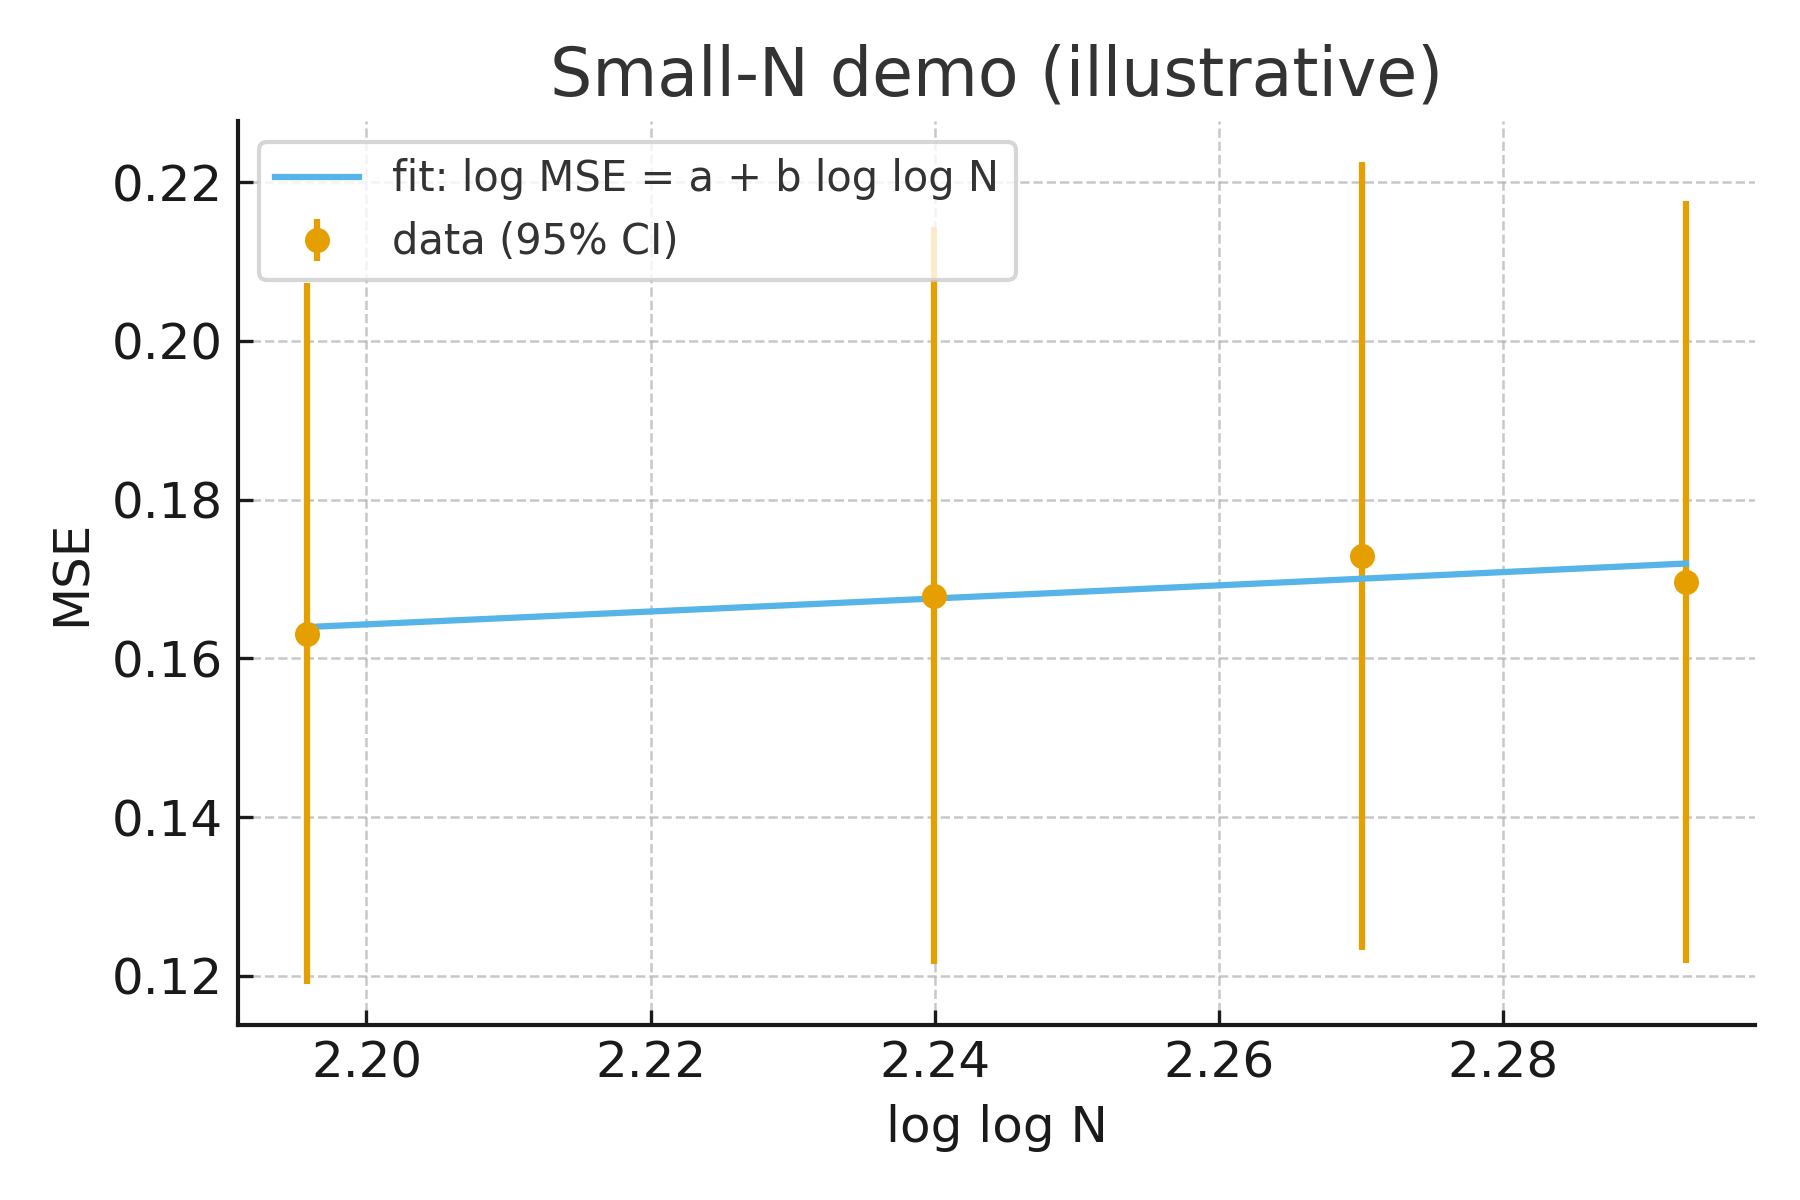
\includegraphics[width=0.8\linewidth]{figures/scaling_smallN.png}
\caption{Small-$N$ demo (illustrative): reported MSE with 95\% CI and OLS fit of $\log(\mathrm{MSE})=\alpha-\theta\log\log N$.
Absolute values are illustrative; large-$N$ claims are \emph{not} made here.}
\label{fig:smallN}
\end{figure}

\section{Scope and Limitations}
Lemma~\ref{lem:hilbert} explains off-diagonal suppression for M\"obius-weighted designs.
It does not establish zero-free regions nor prove RH.
Large-$N$ numerics (beyond this demo) require careful conditioning and are \emph{out of scope} here.

\paragraph{MSC / Keywords.}
MSC: 11M06, 11N37. Keywords: Riemann zeta, Nyman--Beurling, Báez-Duarte, M\"obius, Hilbert kernel.

\section*{Acknowledgments}
The author thanks the community for prior feedback and emphasizes this is a stability-oriented clarification.

\bibliographystyle{plain}
\bibliography{refs}

\end{document}
